% \pdfminorversion=4
\documentclass{beamer}
\usepackage[utf8]{inputenc}
\usepackage{indentfirst}
% \usepackage{enumitem}
\usepackage{datetime2}

\usepackage{textcomp}
\usepackage[T1]{fontenc}
\usepackage{multirow,bigdelim}
\usepackage{float}
\usepackage[caption = false]{subfig}
\usepackage{longtable}
\usepackage{listings}
\usepackage{mathtools}
\DeclareMathOperator{\tr}{Tr}
\usepackage{commath}
\usepackage{slashed}
\usepackage{bbold}
\usepackage{xcolor}
\usepackage{physics}
\newcommand{\lambdabar}{{\mkern0.75mu\mathchar '26\mkern -9.75mu\lambda}}
% \usepackage[right=4cm,left=2cm,top=3cm,bottom=3.0cm, marginparwidth=2.7cm, marginparsep=3mm]{geometry}
\usepackage{mdframed}
\usepackage[version=4]{mhchem}
% \usepackage{tikz} 
% \usetikzlibrary{shapes,arrows,positioning,automata,backgrounds,calc,er,patterns}
% \usepackage{tikz-feynman}

% \tikzfeynmanset{
%   extra large/.style={
%     /tikz/node distance=3cm,
%     /graph drawing/node distance=4cm,
%     /graph drawing/level distance=3cm,
%     /graph drawing/sibling distance=5cm,
%     /tikz/graphs/edges={thick},
%     /tikzfeynman/every dot@@/.append style={/tikz/minimum size=4mm},
%     /tikzfeynman/every crossed dot@@/.append style={/tikz/minimum size=8mm},
%     /tikzfeynman/every blob@@/.append style={/tikz/minimum size=2cm},
%     /tikzfeynman/arrow size=2pt,
%     /tikzfeynman/insertion/size=8pt,
%   },
% }

% \usepackage{simplewick}
% \usepackage{simpler-wick}
% \usetikzlibrary{calc}

%\usepackage{tikz-cd}
\usepackage{amsmath}
\usepackage{amsfonts}
\usepackage{amssymb}
\usepackage{amsthm}
% \numberwithin{equation}{section}
\usepackage{graphicx}
% \usepackage[colorinlistoftodos]{todonotes}
\PassOptionsToPackage{hyphens}{url}
% \usepackage[colorlinks=true, allcolors=blue]{hyperref}
\usepackage{siunitx}
\sisetup{separate-uncertainty=true}
\DeclareSIUnit\erg{erg}
\DeclareSIUnit\parsec{pc}
\DeclareSIUnit\littleh{\textit{h}}
\usepackage{cancel}
\usepackage{mathrsfs}
\usepackage{tensor}
\usepackage{marginnote}
\renewcommand*{\marginnotevadjust}{-0.3cm}
\renewcommand*{\marginfont}{\scriptsize}
% \usepackage{fancybox}

\usepackage{footnotebackref}

\usepackage[sc]{mathpazo}
\linespread{1.05}         % Palladio needs more leading (space between lines)
\usepackage[T1]{fontenc}

\newcommand{\diag}[1]{\text{diag}\qty(#1)}
\newcommand{\const}{\text{const}}
\newcommand{\sign}{\text{sign}}
\renewcommand{\H}{\mathcal{H}}
\renewcommand{\dim}{\text{dim}}
\newcommand{\supp}[1]{\text{supp} \qty(#1)}

% \usepackage{nicefrac}
% \usepackage{ifthen}
% \let\oldfrac\frac
% \renewcommand{\frac}[3][d]{\ifthenelse{\equal{#1}{d}}{\oldfrac{#2}{#3}}{\nicefrac{#2}{#3}}}

\renewcommand{\var}[1]{\text{var} \qty(#1)}
\newcommand{\defeq}{\ensuremath{\stackrel{\text{def}}{=}}}

\newcommand\mybox[1]{%
  \fbox{\begin{minipage}{0.9\textwidth}#1\end{minipage}}}

%Spiegazioni/verifiche
\newenvironment{greenbox}{\begin{mdframed}[hidealllines=true,backgroundcolor=green!20,innerleftmargin=3pt,innerrightmargin=3pt]}{\end{mdframed}}

%Approfondimenti
\newenvironment{bluebox}{\begin{mdframed}[hidealllines=true,backgroundcolor=blue!10,innerleftmargin=3pt,innerrightmargin=3pt]}{\end{mdframed}}

% \newtheorem{claim}{Claim}[section]
% \newtheorem{theorem}{Theorem}[section]
% \newtheorem{definition}{Definition}[section]
% \newtheorem{proposition}{Proposition}[section]

\usepackage{circledsteps}

\newcommand{\hlc}[2]{%
  \colorbox{#1!50}{$\displaystyle#2$}}

\definecolor{codegreen}{rgb}{0,0.6,0}
\definecolor{codegray}{rgb}{0.5,0.5,0.5}
\definecolor{codepurple}{rgb}{0.58,0,0.82}
\definecolor{backcolour}{rgb}{0.95,0.95,0.92}

\lstdefinestyle{mystyle}{
  backgroundcolor=\color{backcolour},
  commentstyle=\color{codegreen},
  keywordstyle=\color{magenta},
  numberstyle=\tiny\color{codegray},
  stringstyle=\color{codepurple},
  basicstyle=\ttfamily\footnotesize,
  breakatwhitespace=false,
  breaklines=true,
  captionpos=b,
  keepspaces=true,
  numbers=left,
  numbersep=5pt,
  showspaces=false,
  showstringspaces=false,
  showtabs=false,
  tabsize=2
}

\lstset{style=mystyle}
% \usepackage{svg}

\usepackage{tikz}
\usetikzlibrary{shapes,arrows,shadows}

% \pagestyle{empty}
\definecolor{uququq}{rgb}{0.25,0.25,0.25}

% \usepackage[activate={true,nocompatibility},final,tracking=true,kerning=true,factor=1100,stretch=10,shrink=10]{microtype}

\newcommand{\boxalign}[2][0.986\textwidth]{
  \par\noindent\tikzstyle{mybox} = [draw=black,inner sep=6pt]
  \begin{center}\begin{tikzpicture}
   \node [mybox] (box){%
    \begin{minipage}{#1}{\vspace{-5mm}#2}\end{minipage}
   };
\end{tikzpicture}\end{center}}

\newcommand{\bigd}[2]{\frac{\mathrm{D} #1}{\mathrm{D} #2}}
\newcommand{\DD}{\mathrm{D}}

% \author{Jacopo Tissino}

\allowdisplaybreaks
\usetheme{Rochester}


\addtobeamertemplate{navigation symbols}{}{%
    \usebeamerfont{footline}%
    \usebeamercolor[fg]{footline}%
    \hspace{1em}%
    \insertframenumber/16
}

\title{Machine Learning \\ for Gravitational Wave data analysis}
\author{Jacopo Tissino\inst{1} \\ 
with Sebastiano Bernuzzi,\inst{2} Matteo Breschi,\inst{2} Rossella Gamba\inst{2}}
\institute{
    \inst{1}Gran Sasso Science Institute
    \and
    \inst{2}TPI, Jena University
}
% with Sebastiano Bernuzzi, Matteo Breschi, Rossella Gamba (JenaU)
\subtitle{Physics of Data workshop}
\date{Venice, 2022-04-08}

\begin{document}

\section{Main presentation}
\frame{\titlepage}

\begin{frame}
    \frametitle{Virgo interferometer}
    \begin{figure}[ht]
        \centering
        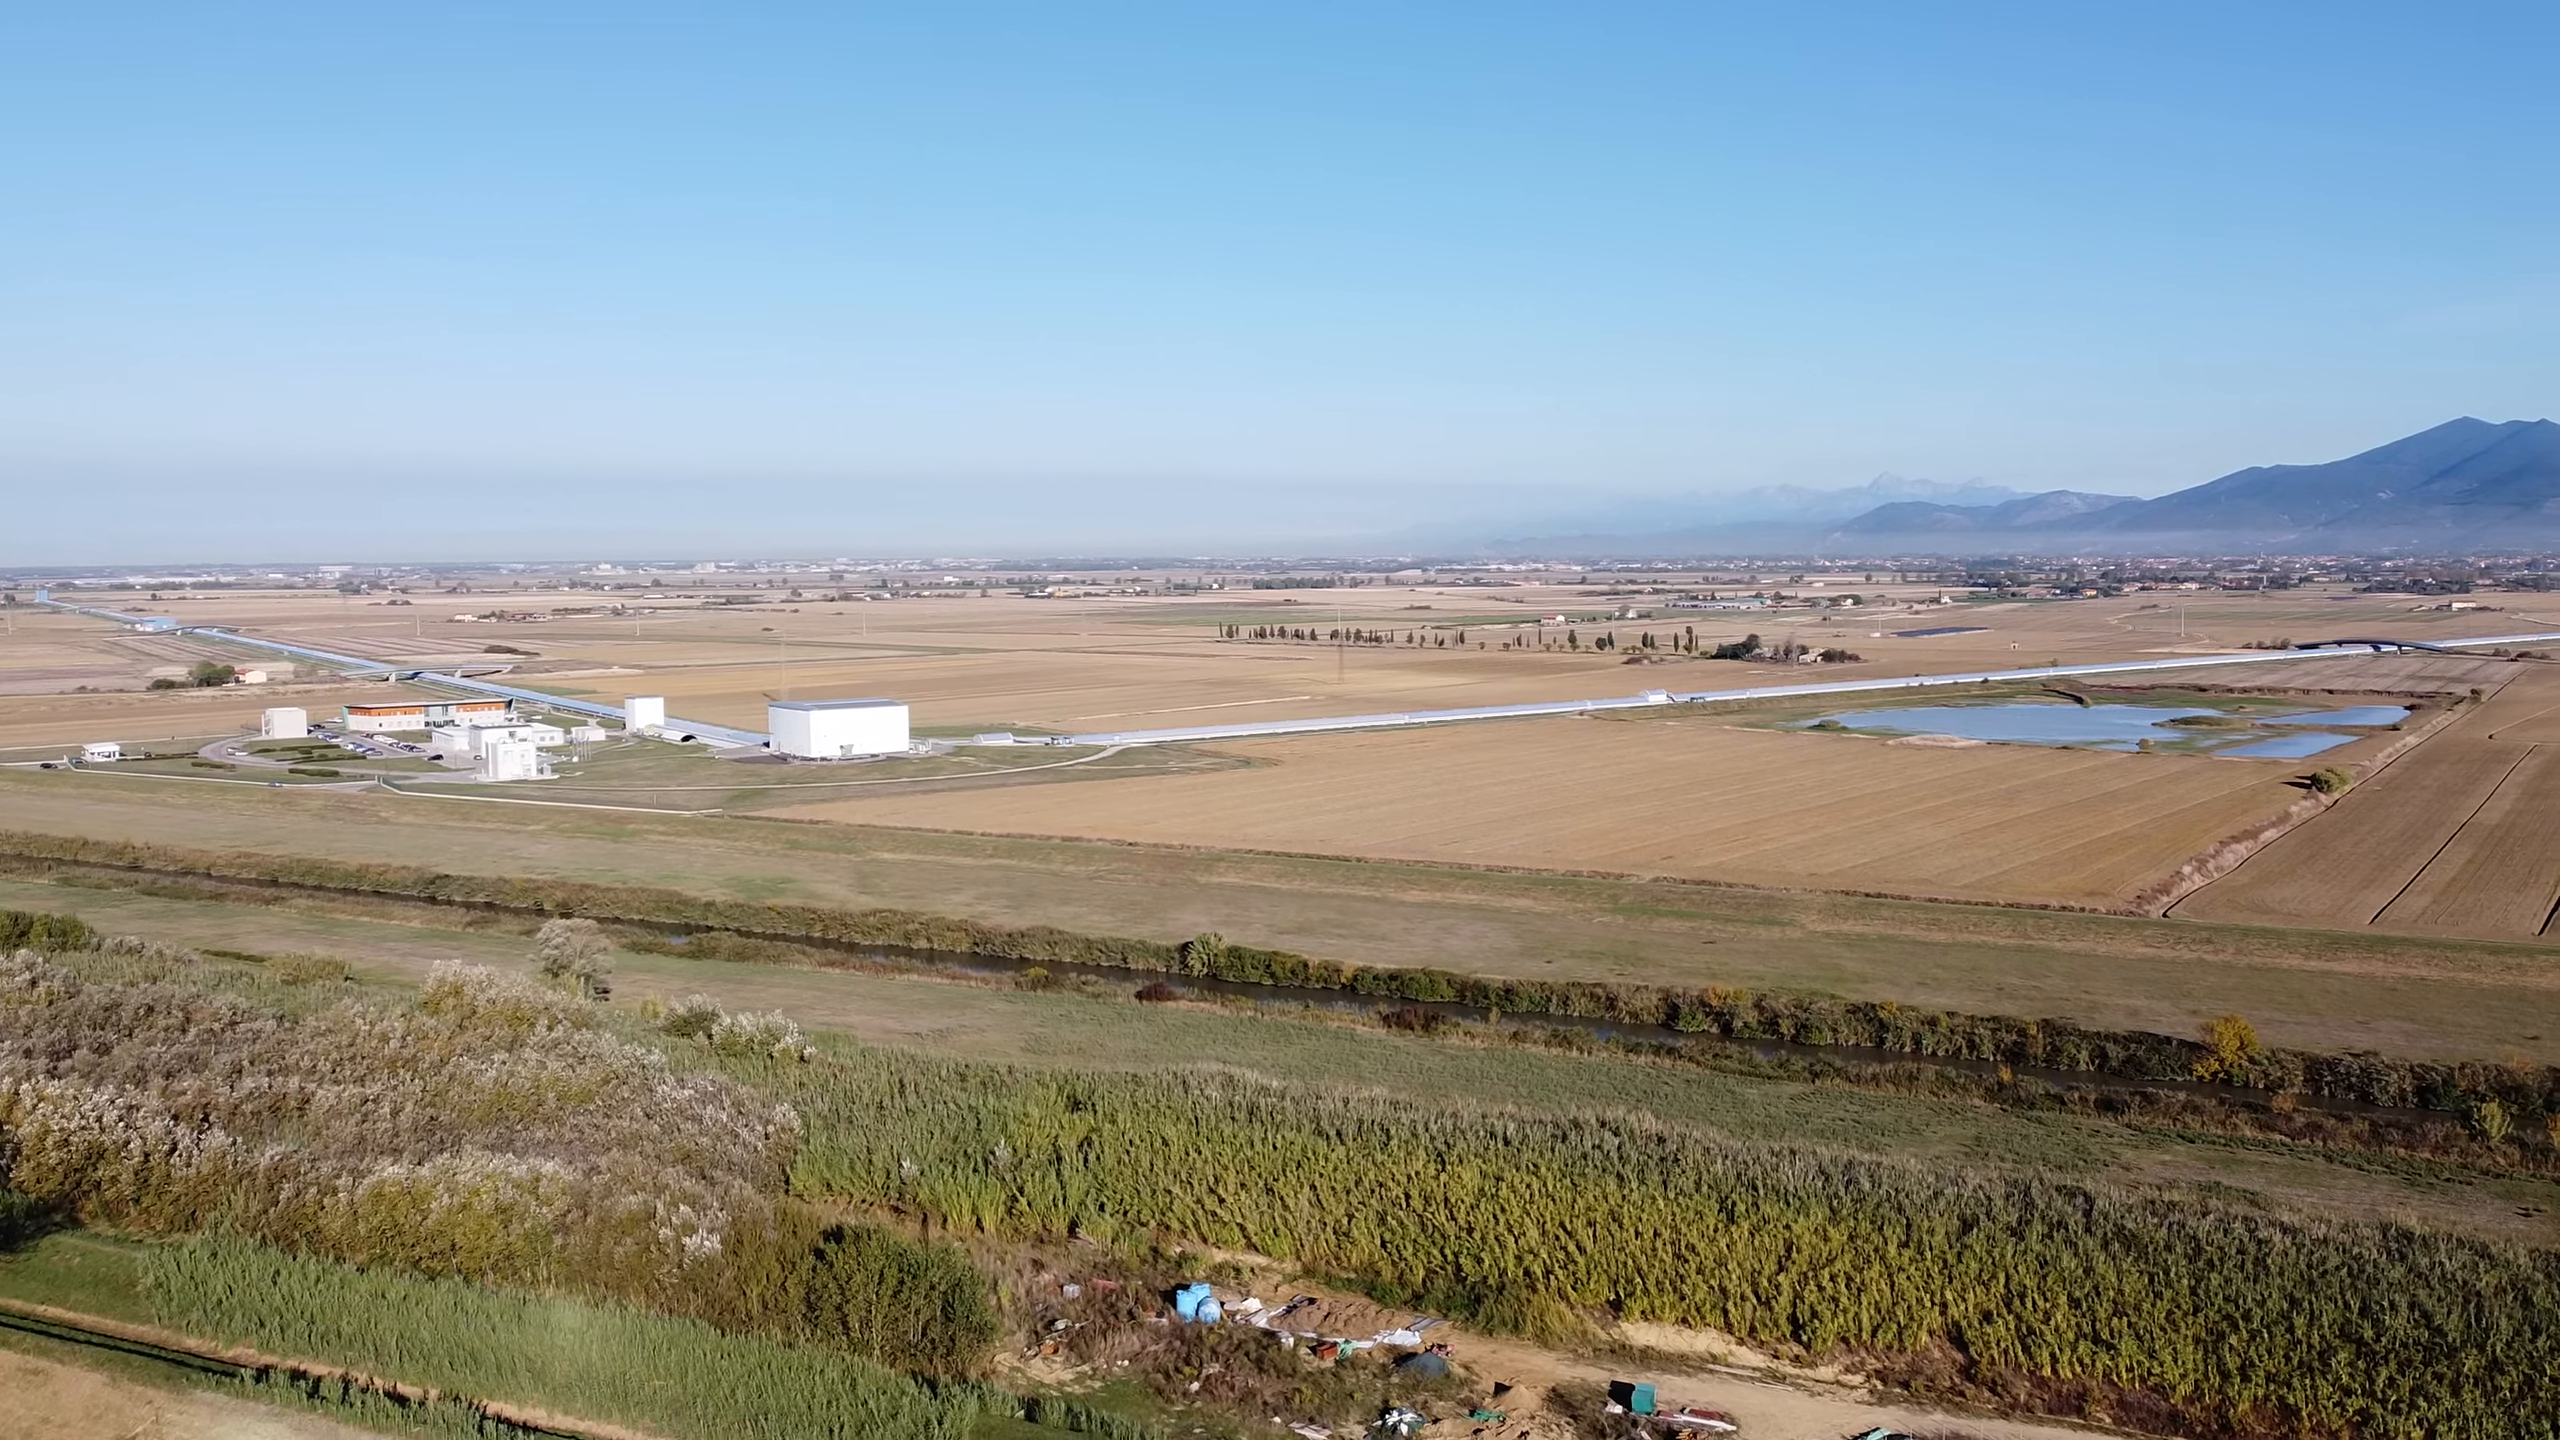
\includegraphics[width=\textwidth]{figures/Virgo}
        \label{fig:Virgo}
    \end{figure}
\end{frame}

\begin{frame}
    \frametitle{Bare interferometer data}
    \begin{figure}[ht]
    \makebox[\textwidth][c]{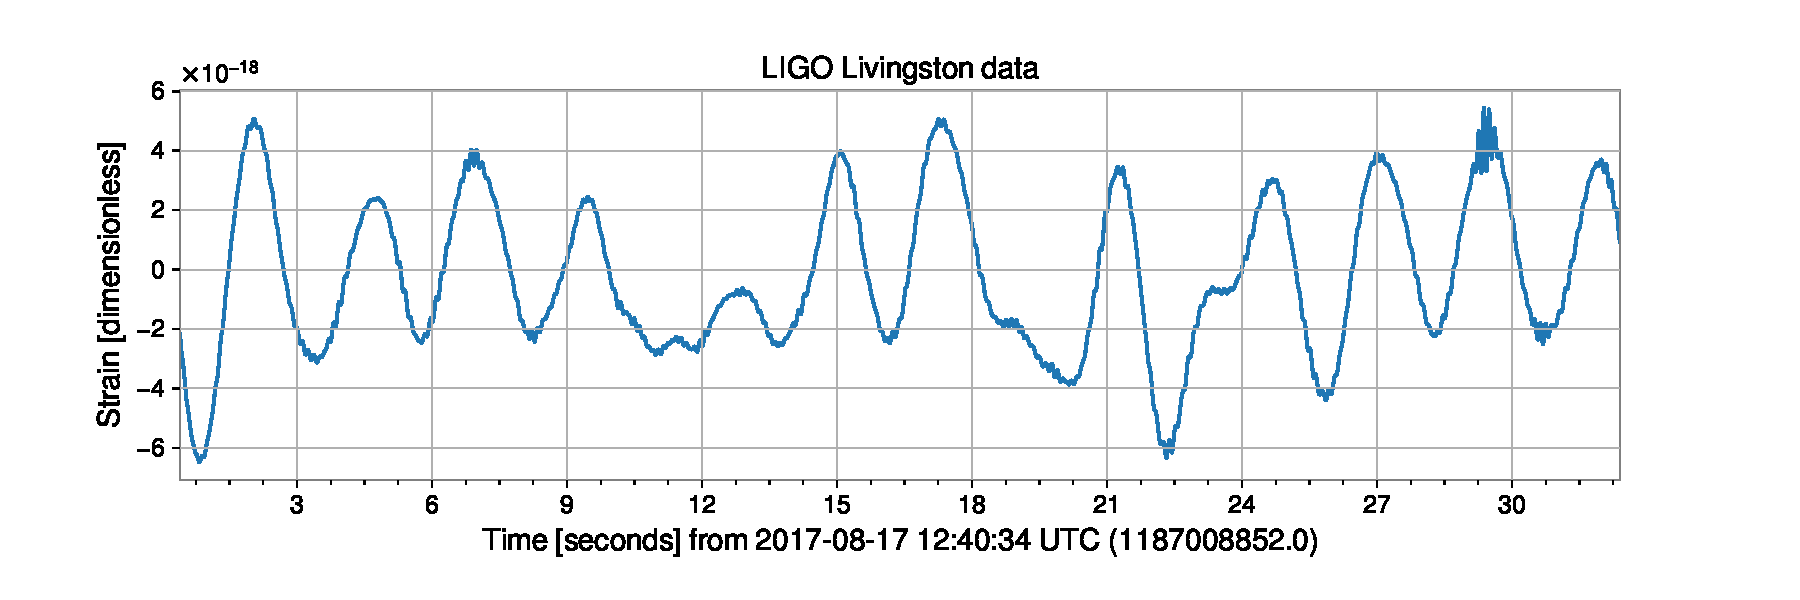
\includegraphics[width=1.3\textwidth]{figures/bare}}
    \label{fig:bare}
    \end{figure}
\end{frame}

\begin{frame}
    \frametitle{Describing Gaussian noise}
    We can completely characterize Gaussian noise through its \textbf{power} or \textbf{amplitude}
    spectral density:
    %
    \begin{align}
    \text{PSD}(f) = S_n (f) = \lim _{T \to \infty} \frac{\abs{\widetilde{d}(f)}^2}{T} 
    \,,
    \end{align}
    \begin{align}
    \text{ASD} (f) = \sqrt{\text{PSD}(f)}
    \,,
    \end{align}
    %
    and then we can whiten the signal as %
    \begin{align}
    \widetilde{d}_w (f) = \frac{\widetilde{d}(f)}{\sqrt{S_n(f)}}
    \,.
    \end{align}
\end{frame}

\begin{frame}
    \frametitle{Amplitude spectral density}
    \vspace{-.2cm}
    \begin{figure}[ht]
    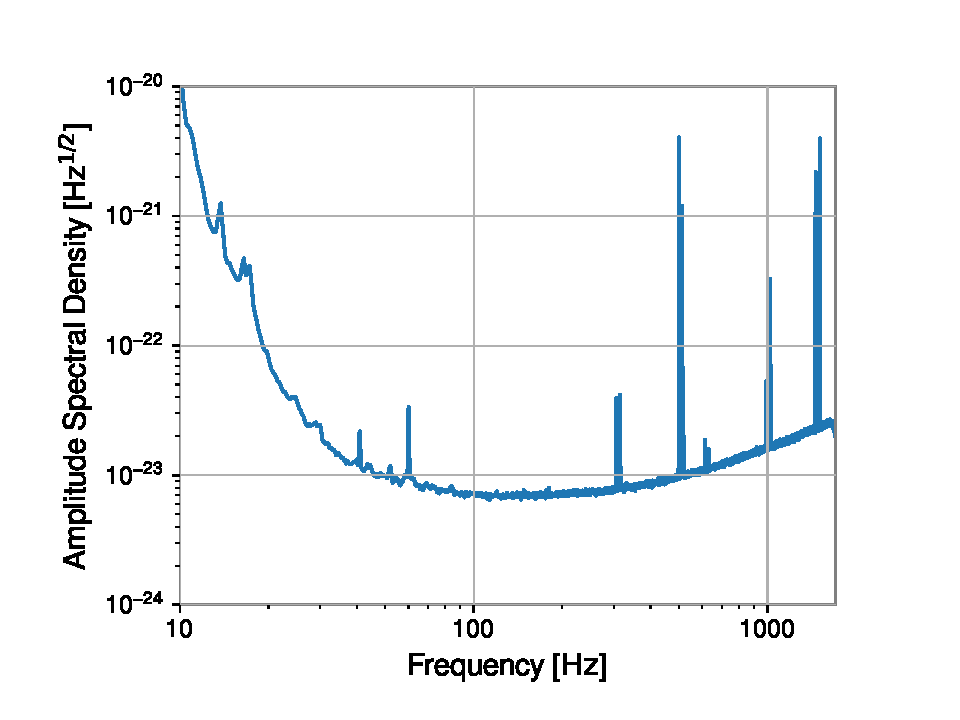
\includegraphics[width=.93\textwidth]{figures/asd}
    \label{fig:asd}
    \end{figure}
\end{frame}

\begin{frame}
    \frametitle{Whitened, bandpassed data}
    \begin{figure}[ht]
    \makebox[\textwidth][c]{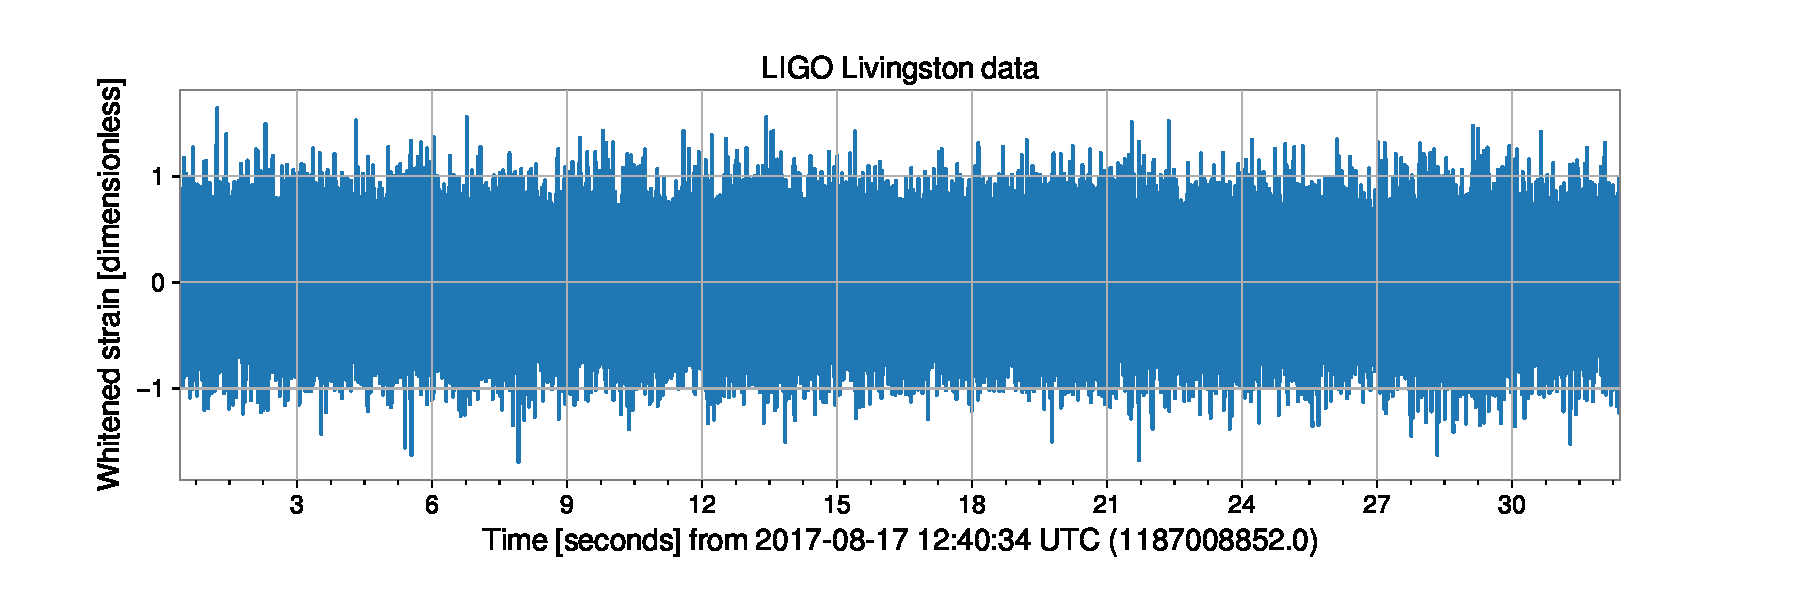
\includegraphics[width=1.3\textwidth]{figures/whitened}}
    \label{fig:whitened}
    \end{figure}
\end{frame}

\begin{frame}
    \frametitle{The signal is small}
    \begin{figure}[ht]    
    \makebox[\textwidth][c]{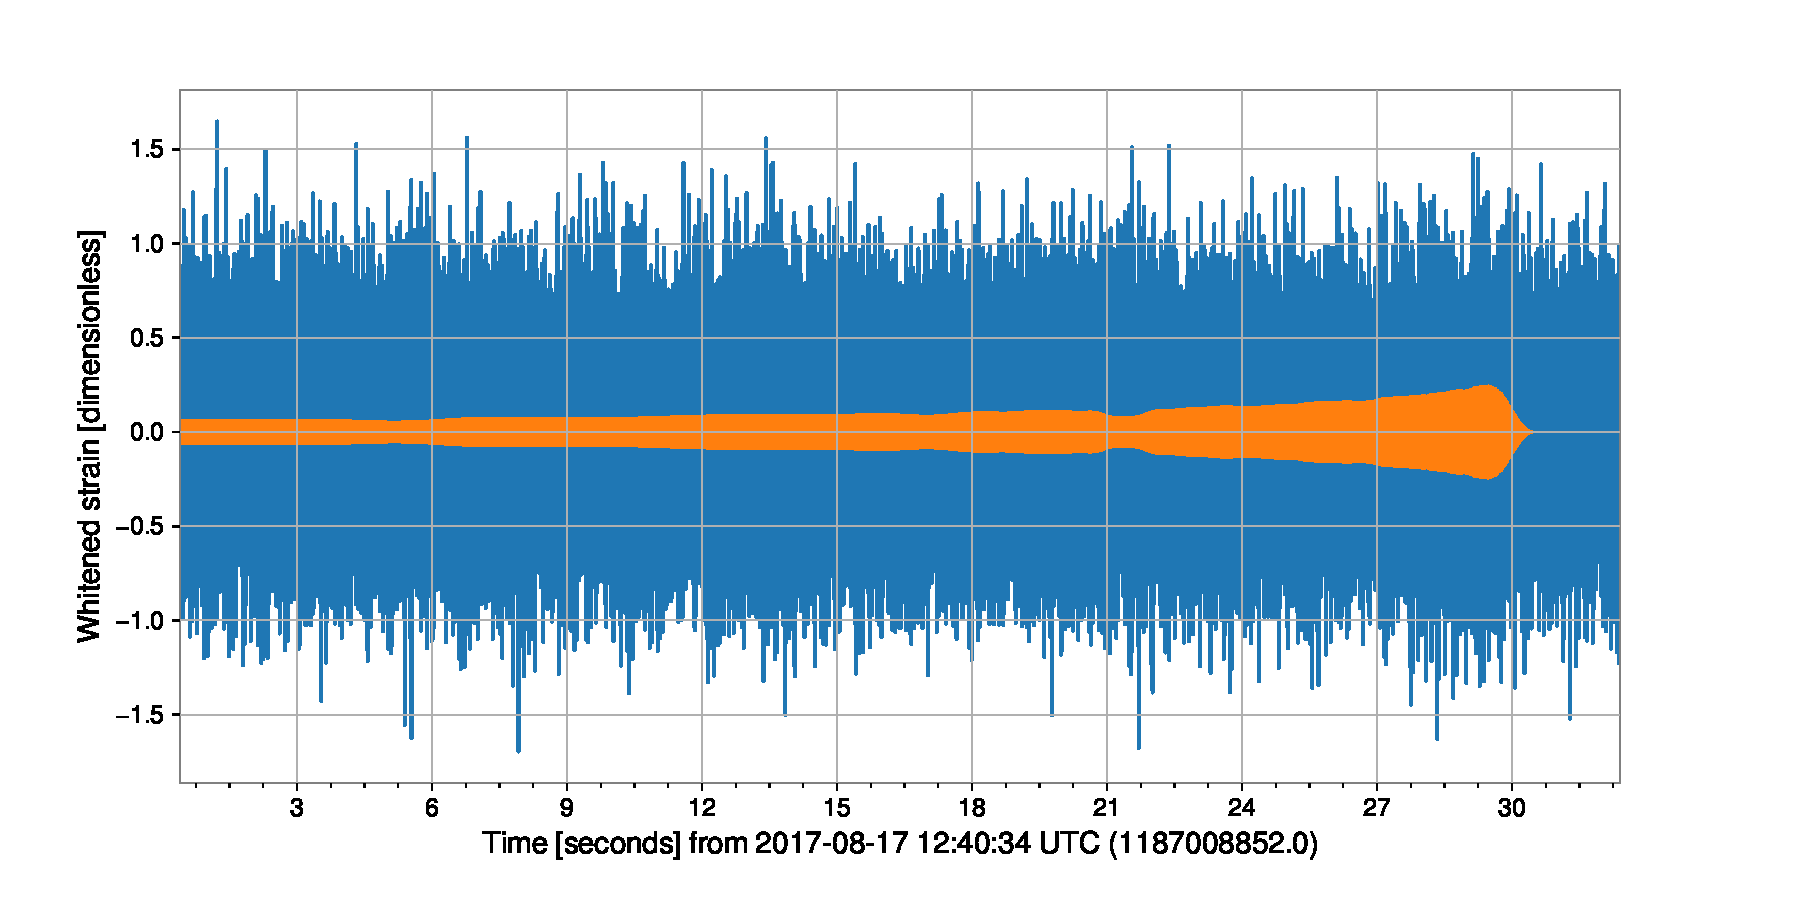
\includegraphics[width=1.25\textwidth]{figures/true_signal}}
    \label{fig:true_signal}
    \end{figure}
\end{frame}

\begin{frame}
    \frametitle{Q-transform}
    \begin{figure}[ht]
    \centering
    \makebox[\textwidth][c]{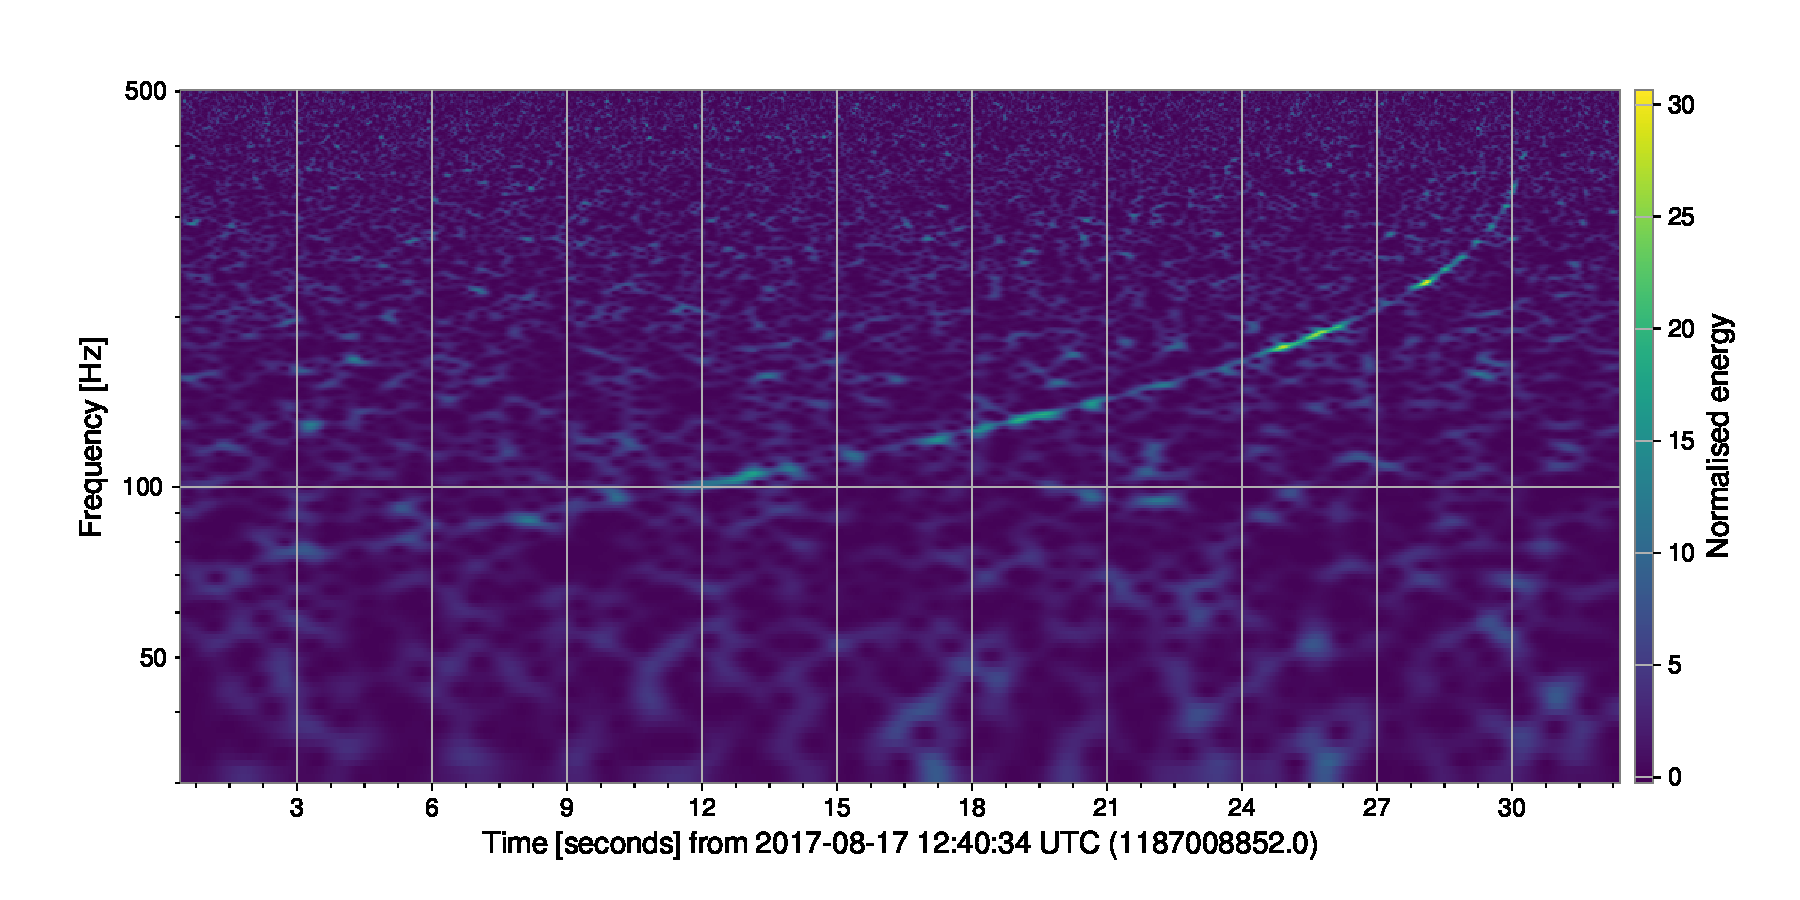
\includegraphics[width=1.2\textwidth]{figures/q_transform}}
    \label{fig:q_transform}
    \end{figure}
\end{frame}


\begin{frame}
    \frametitle{Signal parametrization}
    The strain at the detector is modelled as \(s(t) = h_\theta (t) + n(t)\), where:
    \begin{itemize}
        \item the noise \(n(t)\) is taken to be stationary, with zero mean, and Gaussian with power spectral density \(S_n(f)\);
        \item the signal \(h_\theta (t)\) can depend on: 
        \begin{itemize}
            \item intrinsic parameters: total mass \(M = m_1 + m_2 \), mass ratio \(q = m_1 / m_2 \), spins \(\vec{\chi}_{1}\) and \(\vec{\chi}_2\), tidal polarizabilities \(\Lambda_1\) and \(\Lambda_2 \);
            \item extrinsic parameters: luminosity distance \(D_L\), inclination \(\iota \)\dots
        \end{itemize}
    \end{itemize}
\end{frame}

\begin{frame}
    \frametitle{The Wiener distance}
    
    The likelihood used in parameter estimation reads:
    %
    \begin{align}
        \Lambda (s | \theta ) \propto \exp( (h_\theta | s) - \frac{1}{2} (h_\theta | h_\theta ))
        \,,
    \end{align}
    %
    where \((a | b)\) is the Wiener product: 
    %
    \begin{align}
    (a | b) = 4 \Re \int_{0}^{\infty } \frac{\widetilde{a}^{*}(f) \widetilde{b} (f)}{S_n (f)} \dd{f}
    = 4 \Re \int_0^{ \infty } a_w^* (f) b_w(f) \dd{f}
    \,.
    \end{align}
\end{frame}

\begin{frame}
    \frametitle{A posterior distribution: GW170817}
    \begin{figure}[ht]
    \vspace{-.2cm}
    \centering
    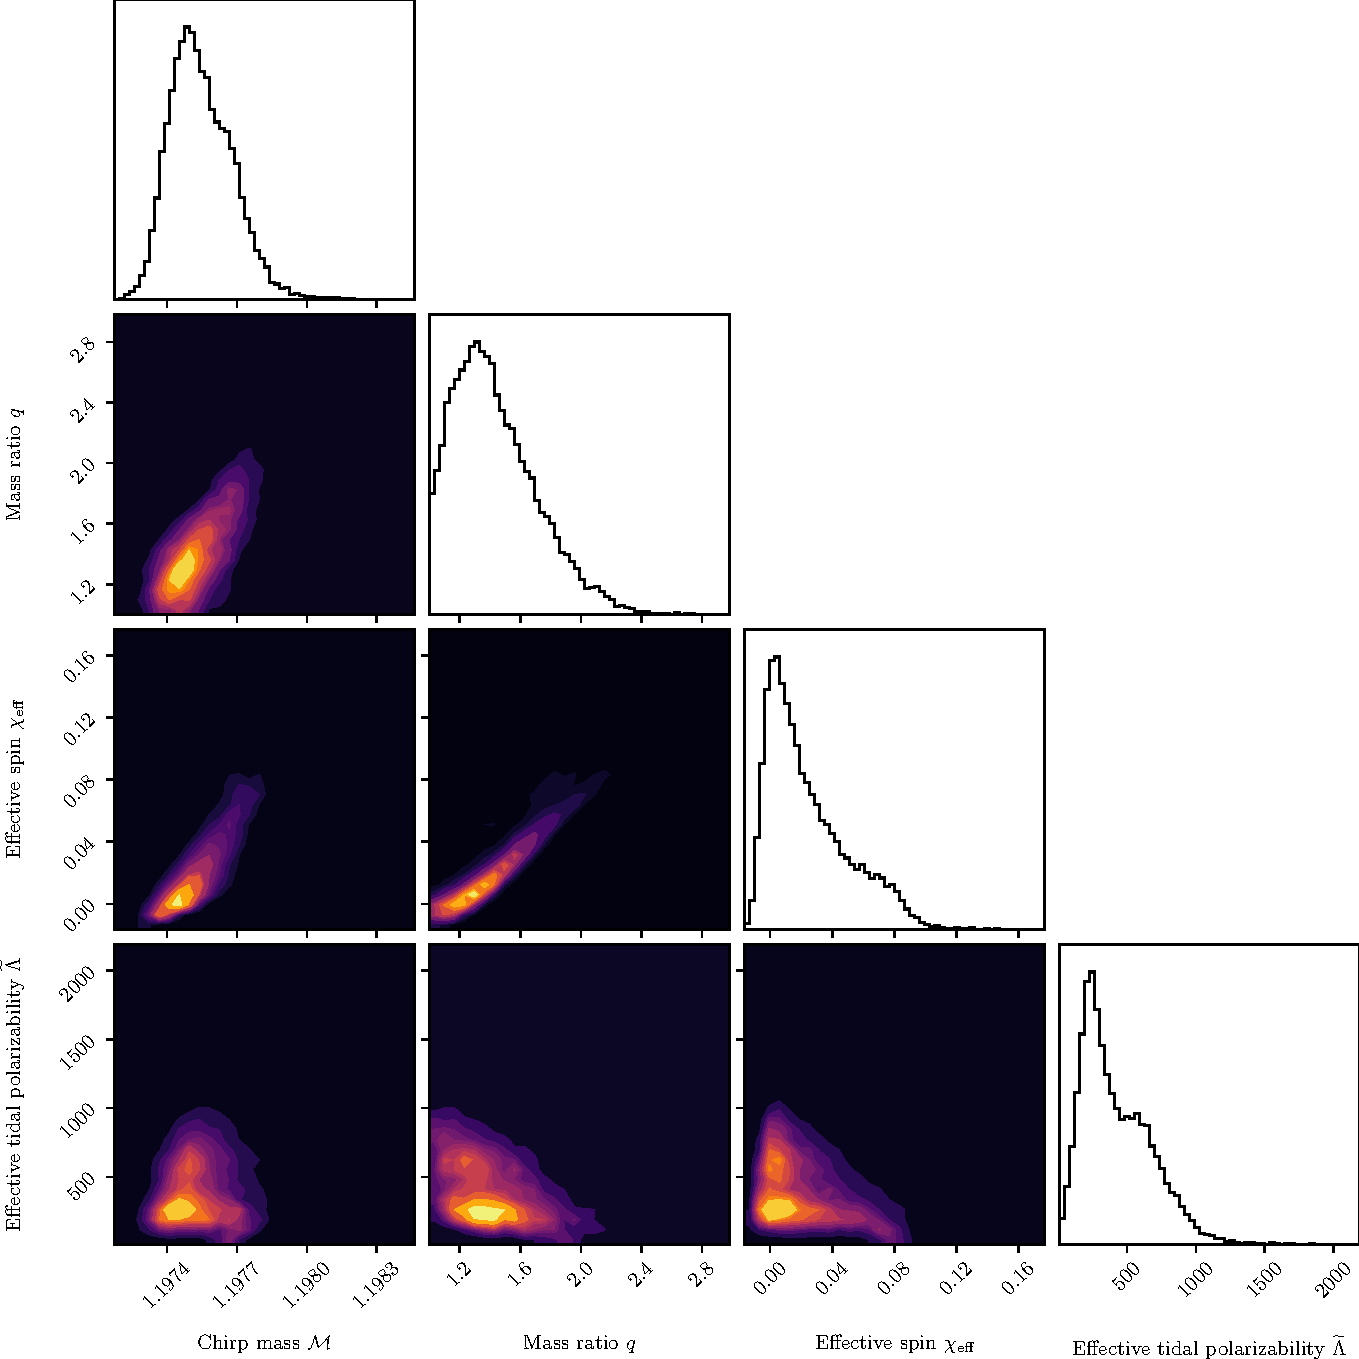
\includegraphics[width=.7\textwidth]{figures/corner_posterior}
    \label{fig:corner_posterior}
    \end{figure}
\end{frame}

\begin{frame}
    \frametitle{Theoretical signal models}
    The main strategies for the generation of theoretical waveforms are: 
    \begin{itemize}
        \item numerical relativity;
        \item effective one body;
        \item post-Newtonian.
    \end{itemize}

    Other methods mix and match these: hybrid waveforms, phenomenological models, 
    \textbf{surrogates}.
\end{frame}

\begin{frame}
    \frametitle{\texttt{mlgw\_bns} structure}
    \vspace*{-.3cm}
    \begin{figure}[ht]
    \centering
    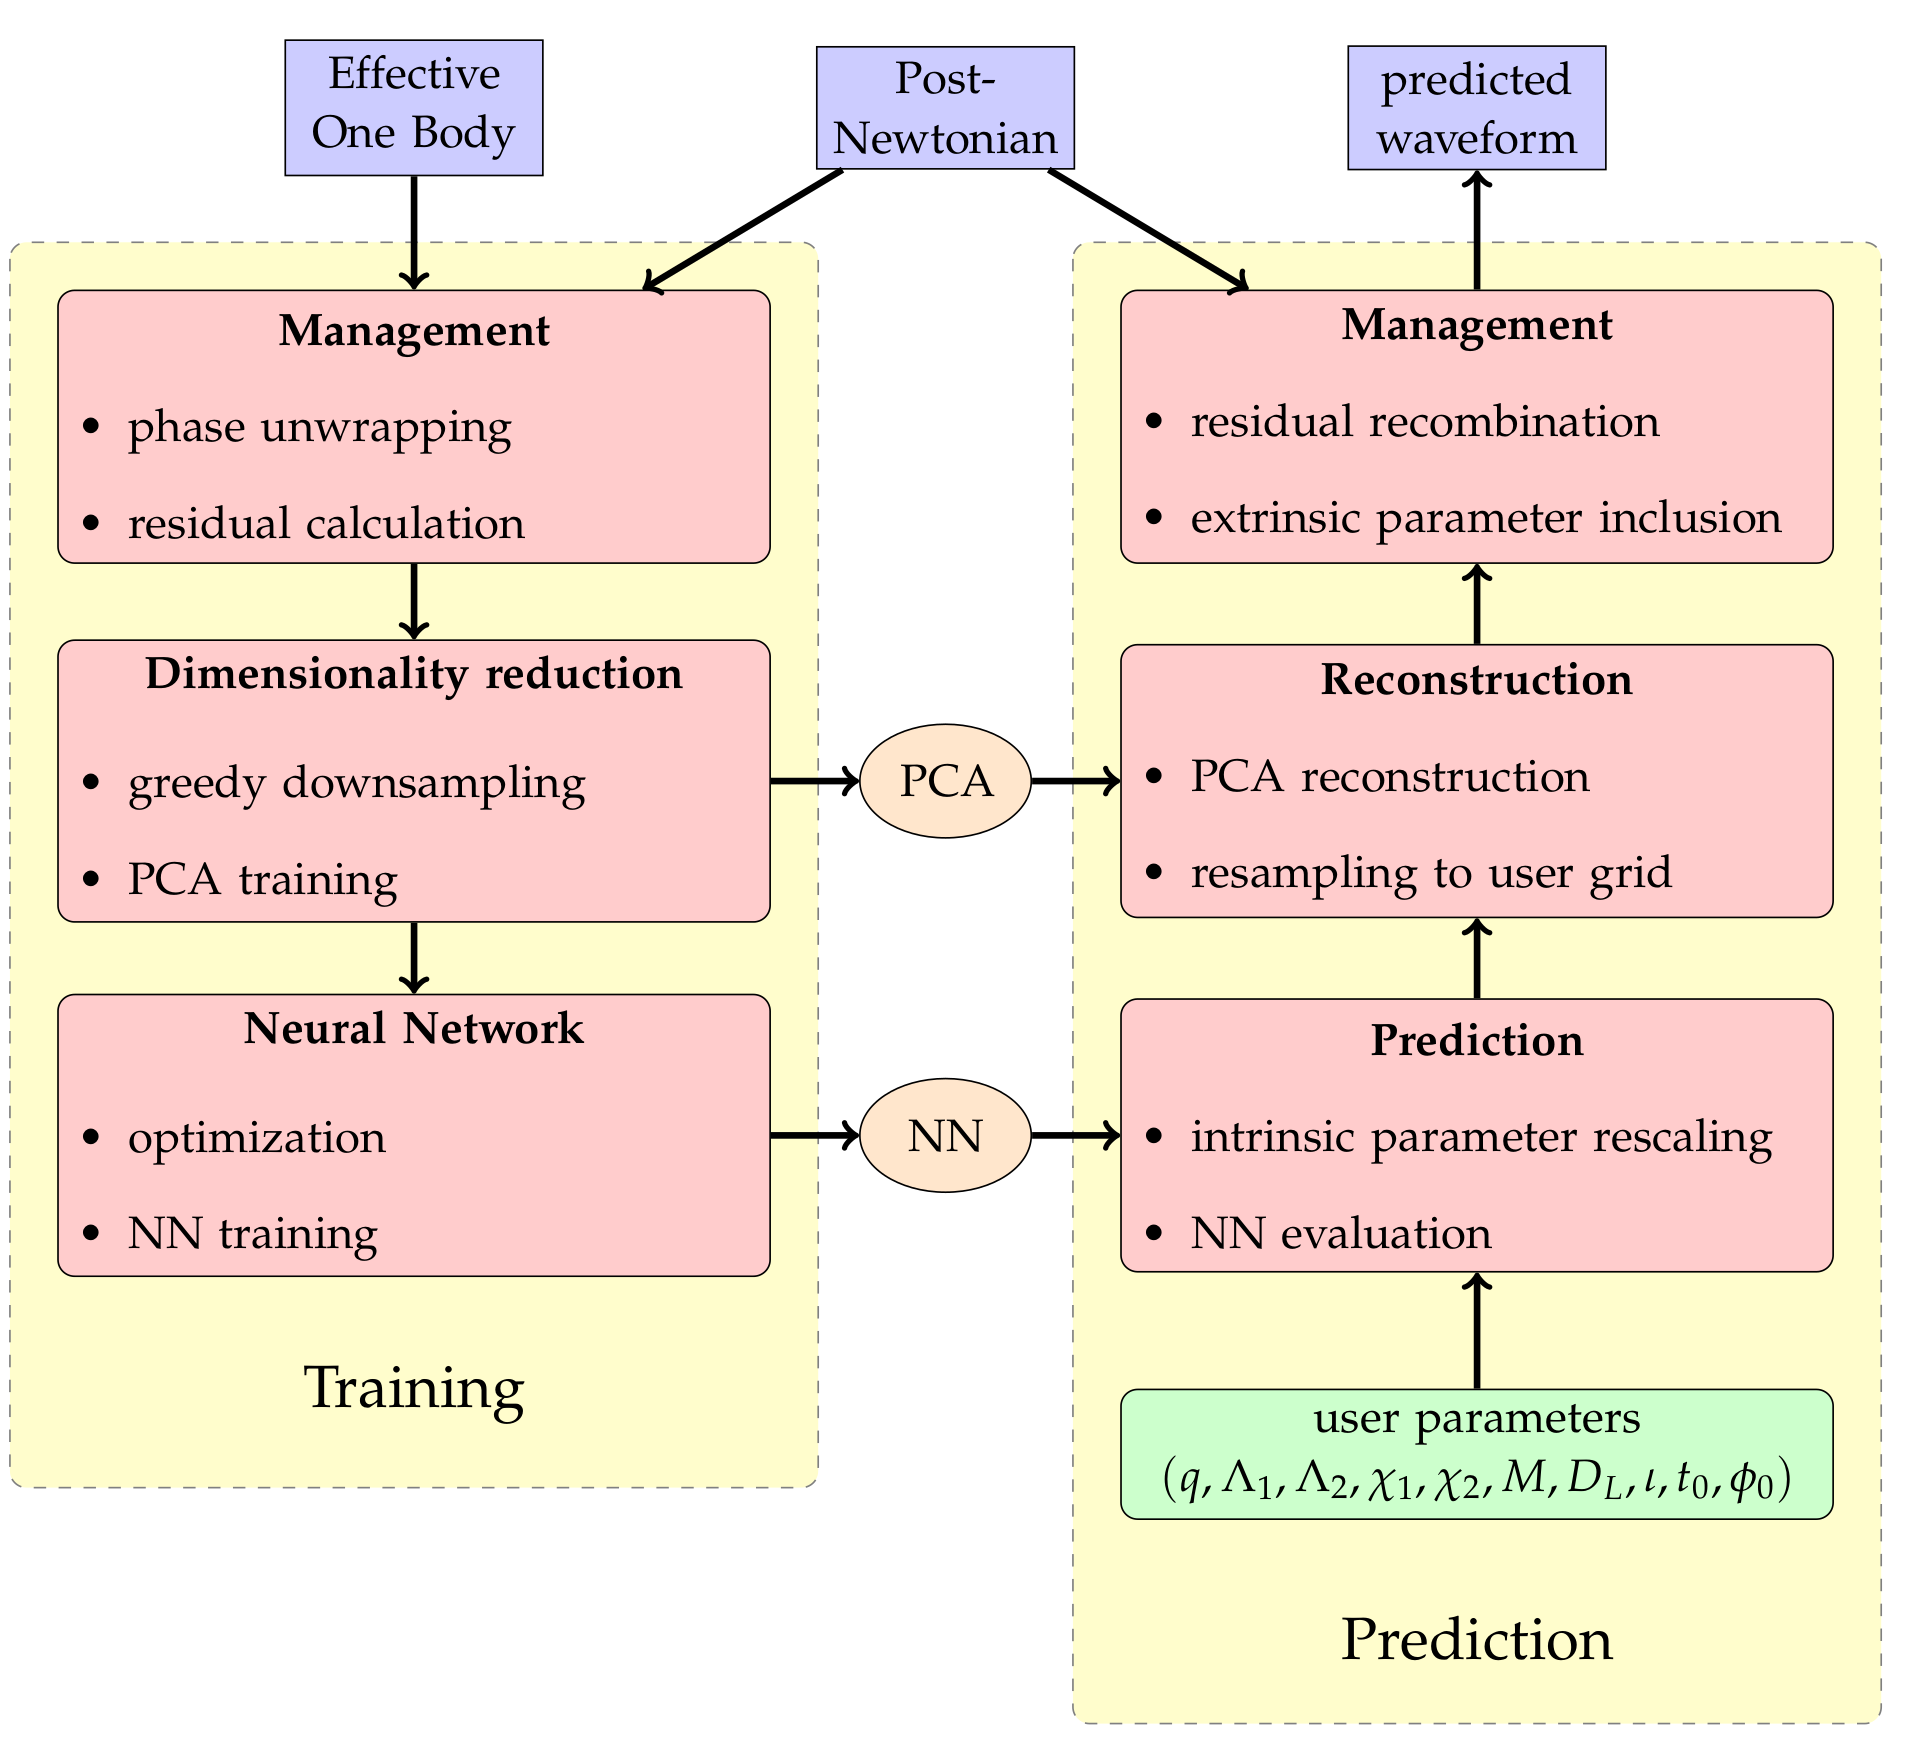
\includegraphics[width=.775\textwidth]{figures/flowchart}
    \label{fig:flowchart}
    \end{figure}
\end{frame}

\begin{frame}
    \frametitle{Evaluation time}
    \begin{figure}[ht]
    \centering
    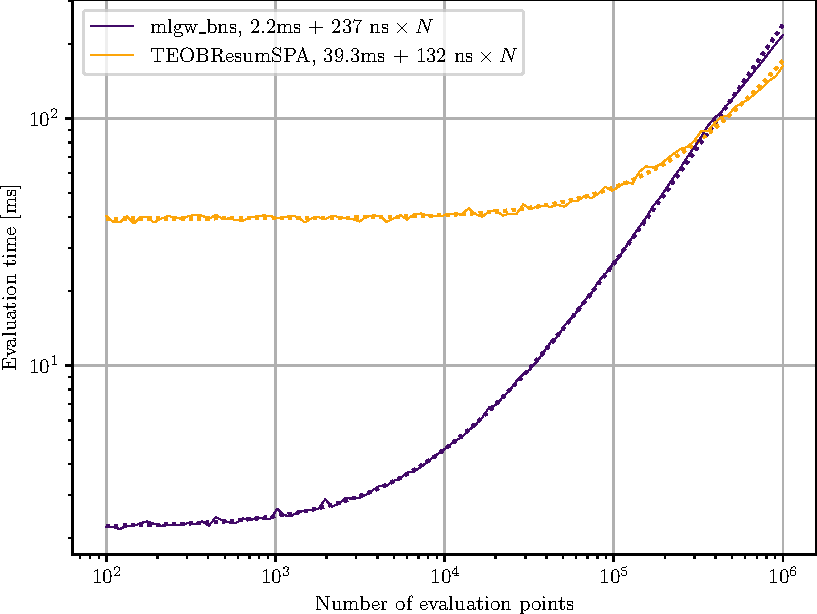
\includegraphics[width=.85\textwidth]{figures/benchmarking_evaluation}
    \label{fig:benchmarking_evaluation}
    \end{figure}
\end{frame}

\begin{frame}
    \frametitle{Fidelity}
    \begin{figure}[ht]
    \centering
    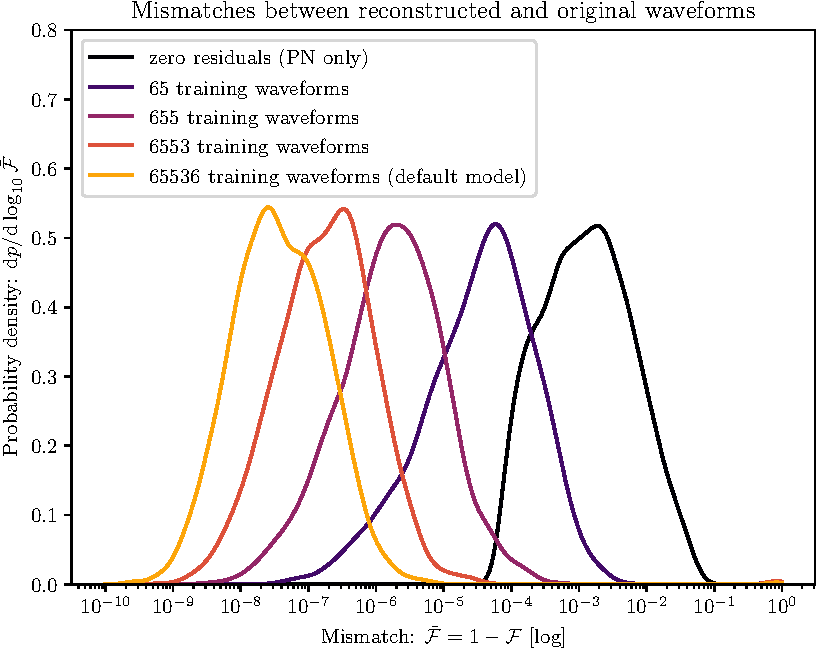
\includegraphics[width=.85\textwidth]{figures/mismatches_by_n_train}
    \end{figure}
\end{frame}

\begin{frame}
    \frametitle{More information}
    \begin{itemize}
        \item Learn about GW data analysis at \url{gw-openscience.org};
        \item documentation for \texttt{mlgw\_bns} is available at \url{mlgw-bns.readthedocs.io};
        \item scripts and source for this presentation are available at \url{github.com/jacopok/pod-workshop}.
    \end{itemize}
\end{frame}

\section{Backup slides}

\begin{frame}
    \frametitle{Technologies}
    \texttt{mlgw\_bns} is implemented as a \texttt{python} package, and it makes use of 
    \begin{itemize}
        \item \texttt{scikit-learn} for the neural network (upgrading to \texttt{pytorch});
        \item \texttt{optuna} for the hyperparameter optimization;
        \item \texttt{pytest} and \texttt{tox} for automated testing;
        \item \texttt{numba} for just-in-time compilation and acceleration.
    \end{itemize}
\end{frame}

\begin{frame}
    \frametitle{Original residuals}
    \begin{figure}[ht]
    \centering
    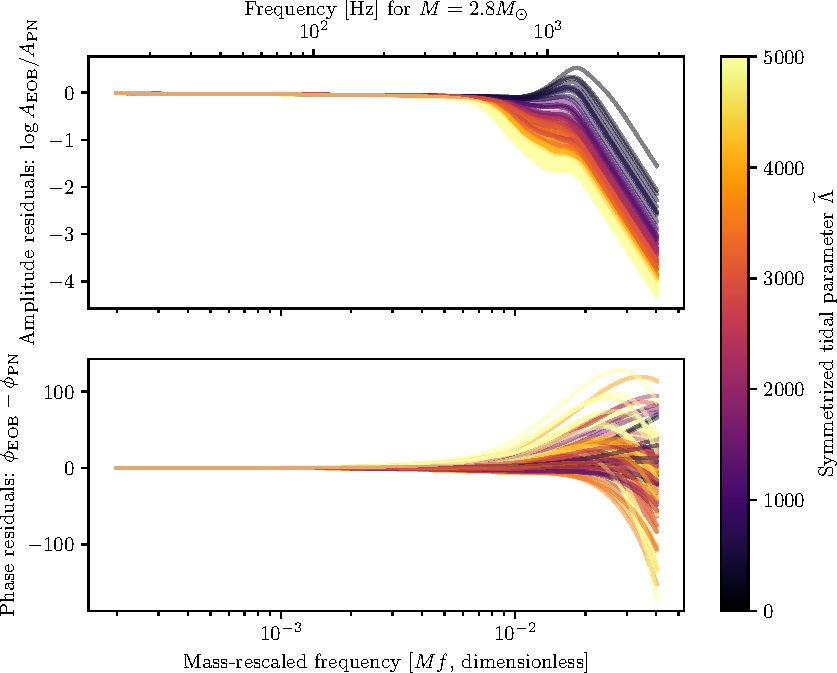
\includegraphics[width=.85\textwidth]{figures/original_residuals}
    \label{fig:original_residuals}
    \end{figure}
\end{frame}


\begin{frame}
    \frametitle{Reconstruction residuals}
    \begin{figure}[ht]
    \centering
    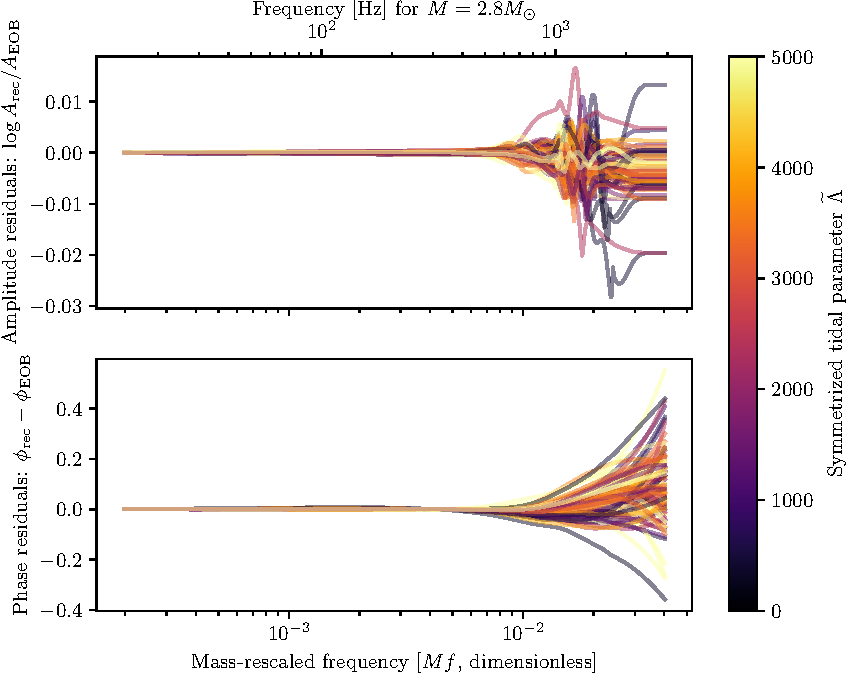
\includegraphics[width=.85\textwidth]{figures/reconstruction_residuals}
    \label{fig:reconstruction_residuals}
    \end{figure}
\end{frame}


\begin{frame}
    \frametitle{Profiling the evaluation: \(\num{8e3}\) interpolation points}
    \begin{figure}[ht]
    \centering
    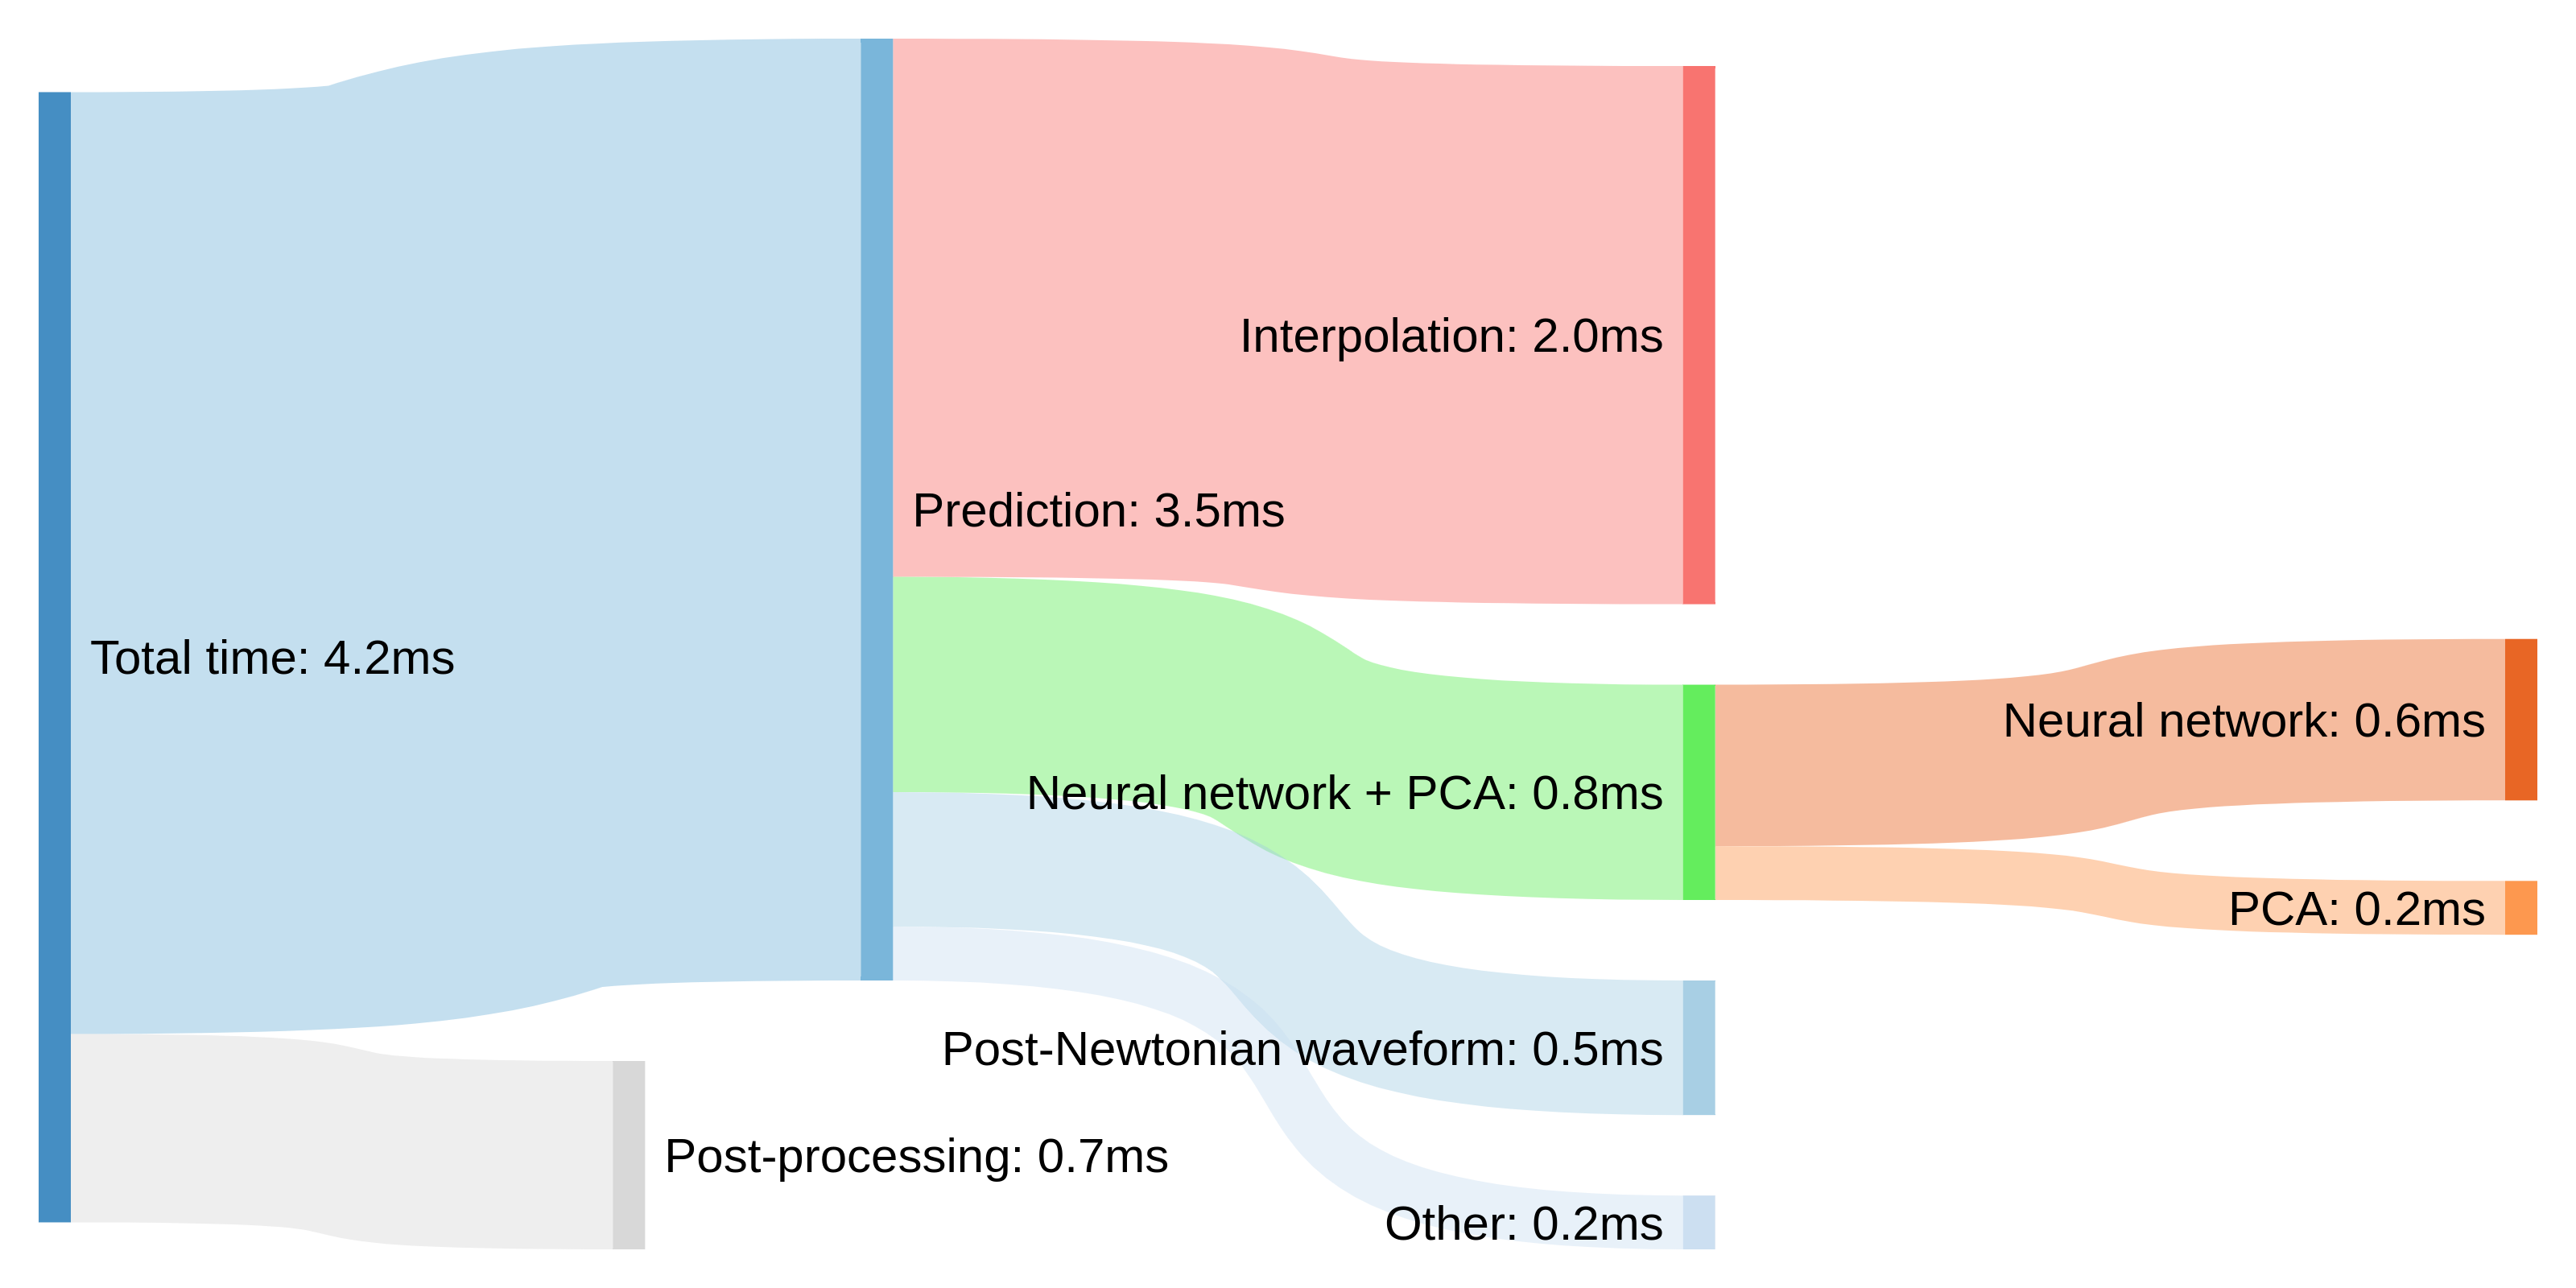
\includegraphics[width=\textwidth]{figures/sankey_downsampled}
    \label{fig:sankey_downsampled}
    \end{figure}
\end{frame}

\begin{frame}
    \frametitle{Profiling the evaluation: \(\num{2e6}\) interpolation points}
    \begin{figure}[ht]
    \centering
    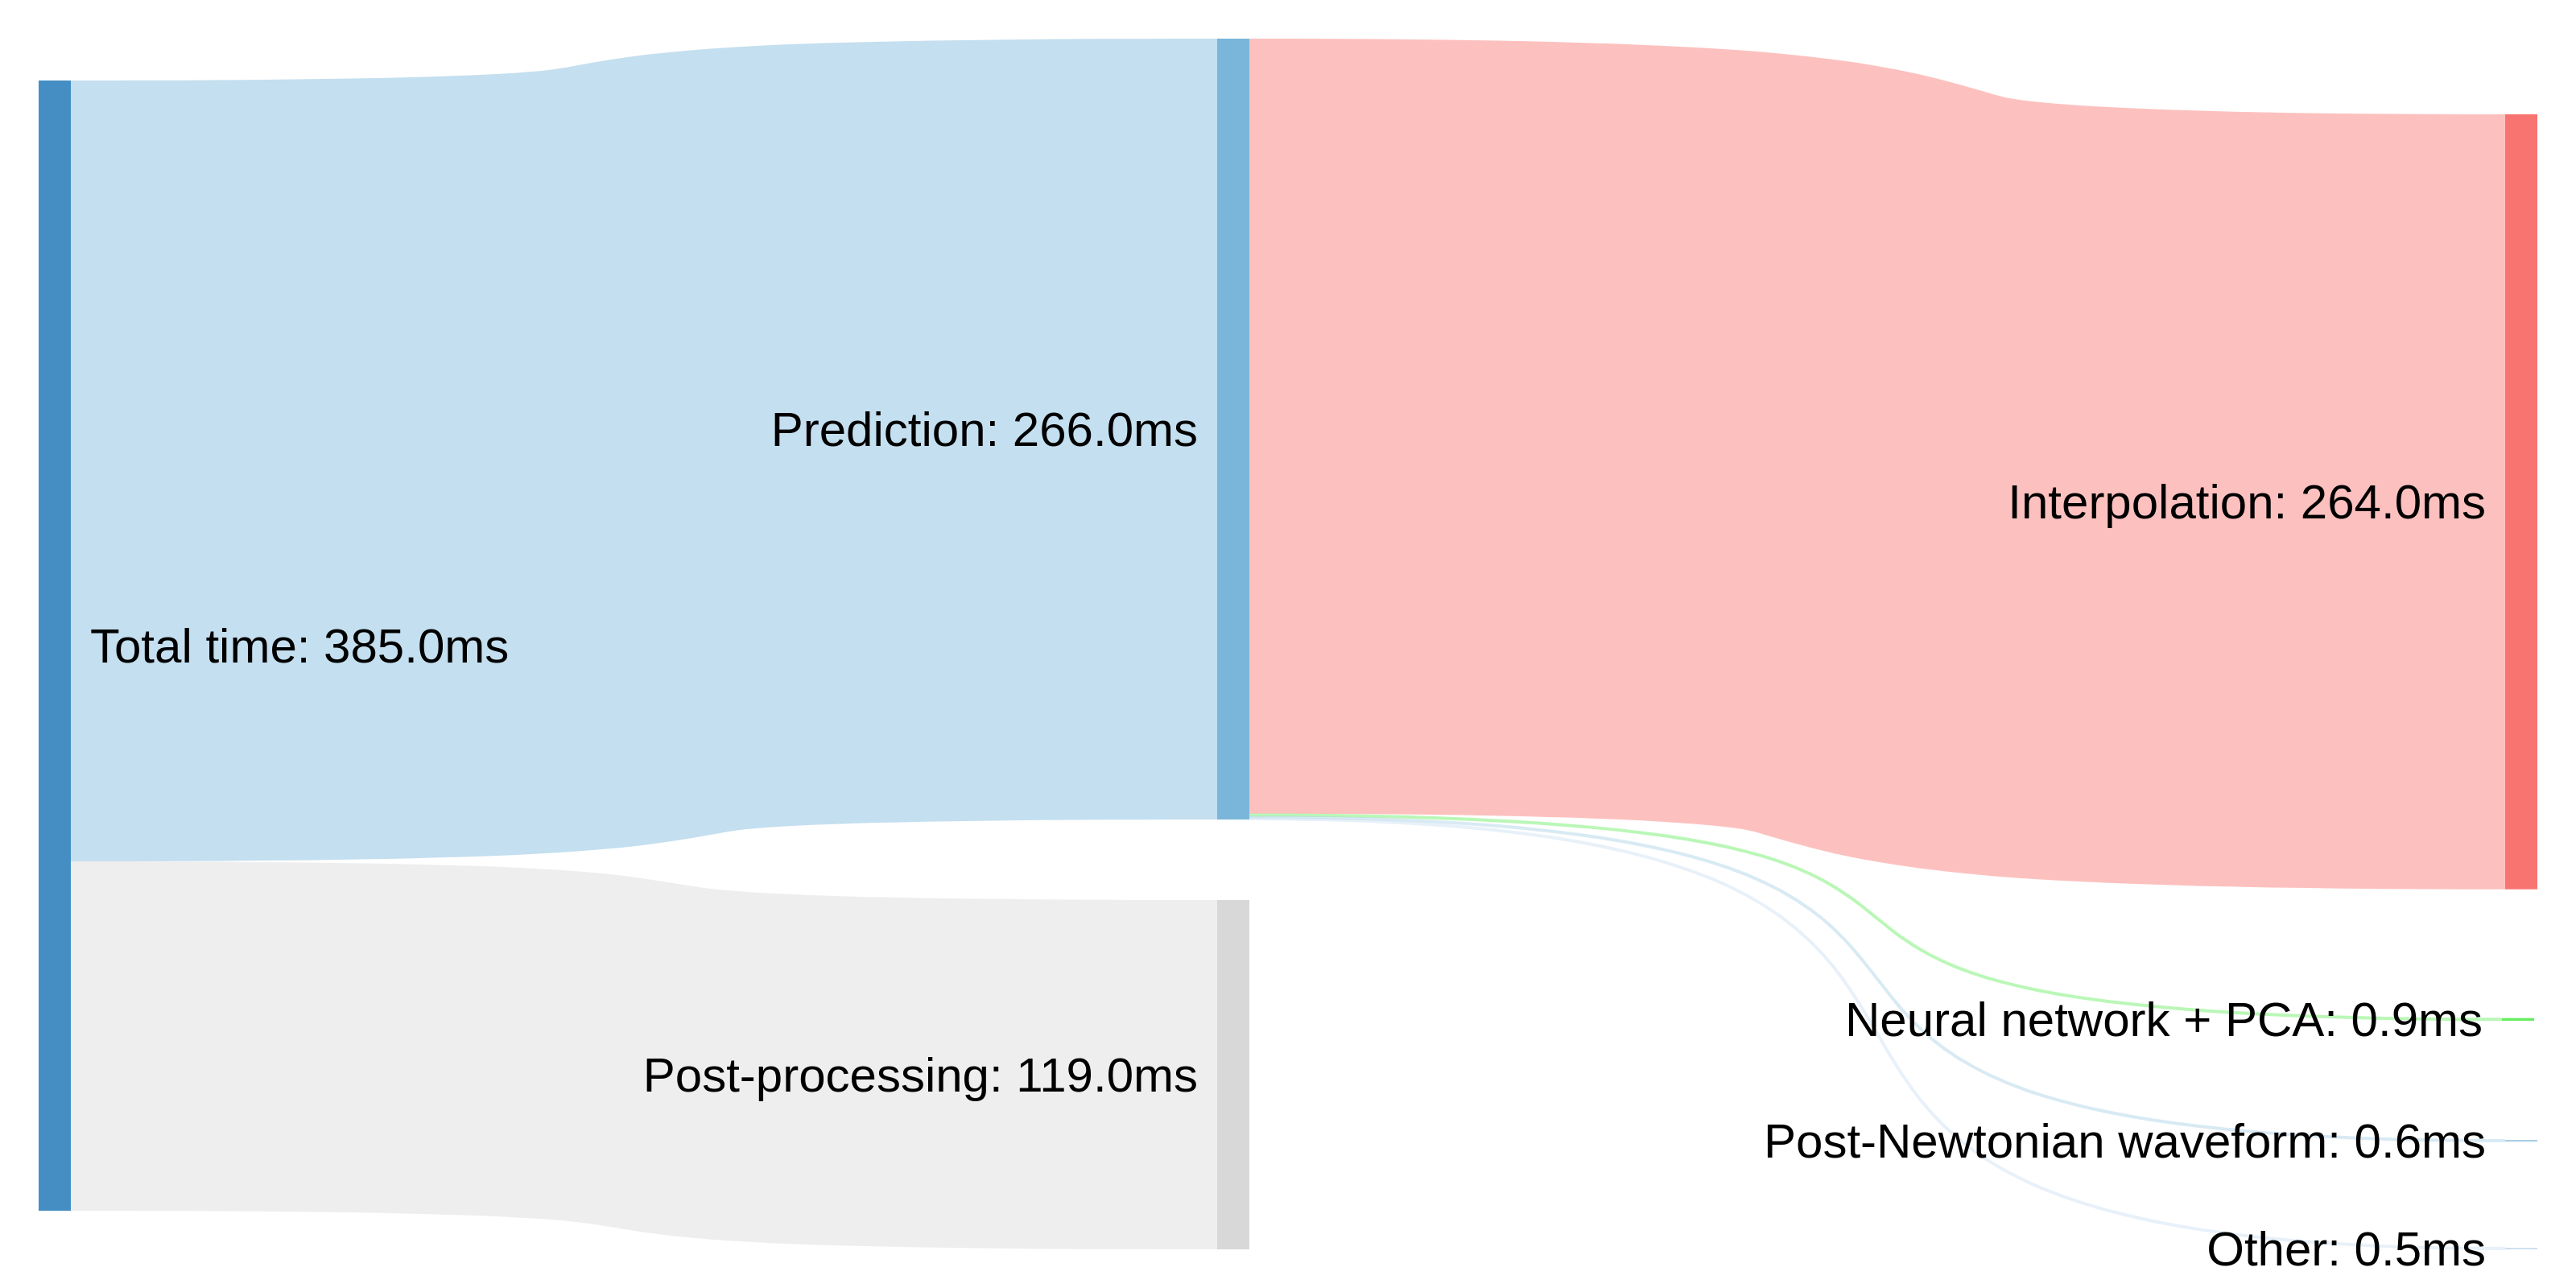
\includegraphics[width=\textwidth]{figures/sankey_full}
    \label{fig:sankey_full}
    \end{figure}
\end{frame}

\begin{frame}
    \frametitle{Hyperparameter optimization}
    \begin{figure}[ht]
    \centering
    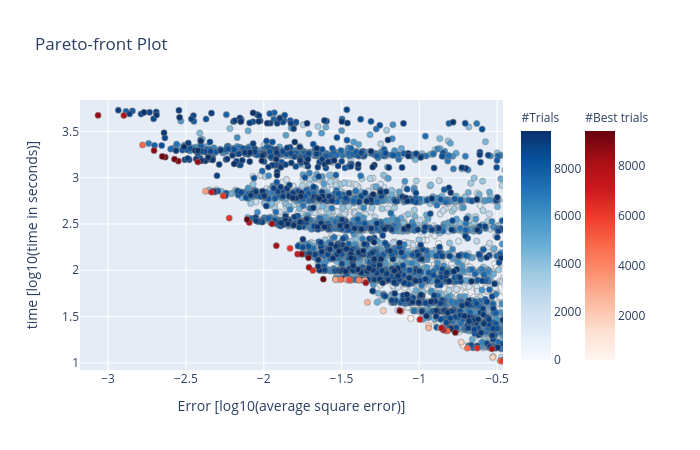
\includegraphics[width=.95\textwidth]{figures/pareto-front}
    \label{fig:pareto-front-nonspinning}
    \end{figure}
\end{frame}

\begin{frame}
    \frametitle{Power Spectral densities and GW170817}
    \begin{figure}[ht]
    \centering
    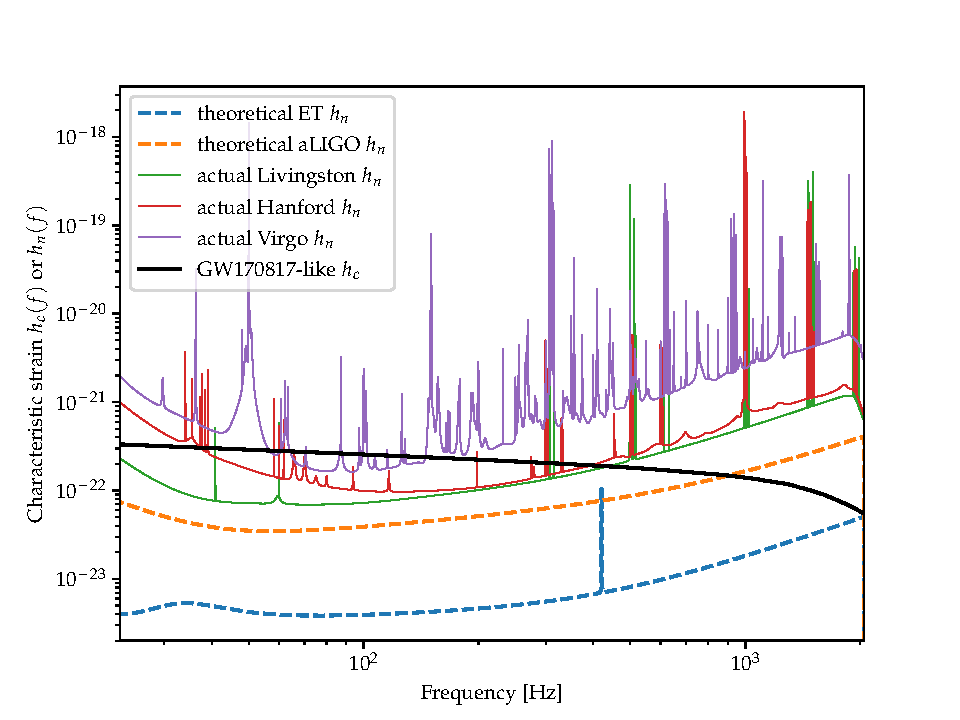
\includegraphics[width=.91\textwidth]{figures/characteristic_strains}
    \label{fig:characteristic_strains}
    \end{figure}
\end{frame}

\begin{frame}
    \frametitle{Amplitudes}
    \begin{figure}[ht]
    \centering
    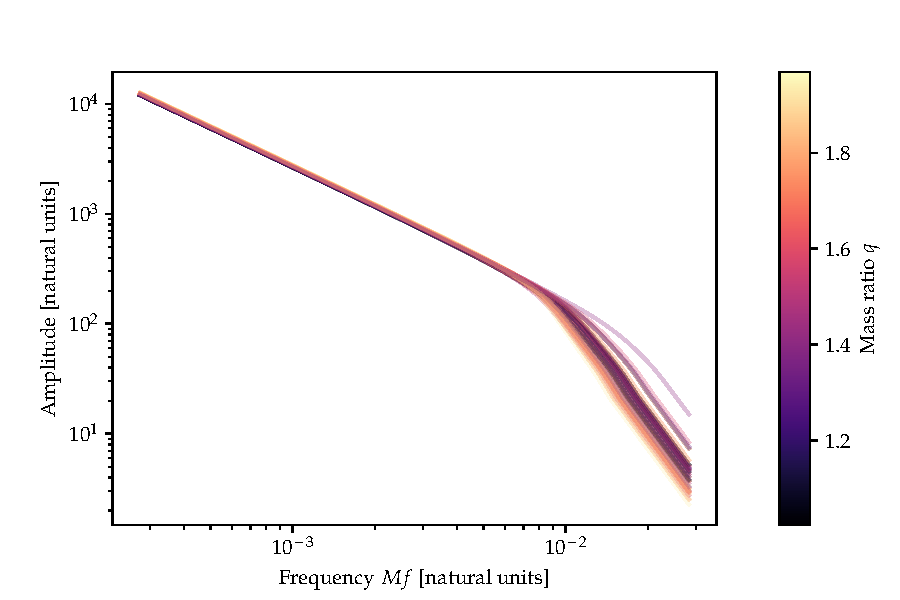
\includegraphics[width=.95\textwidth]{figures/native_amplitudes}
    \label{fig:native_amplitudes}
    \end{figure}
\end{frame}

\begin{frame}
    \frametitle{Phases}
    \begin{figure}[ht]
    \centering
    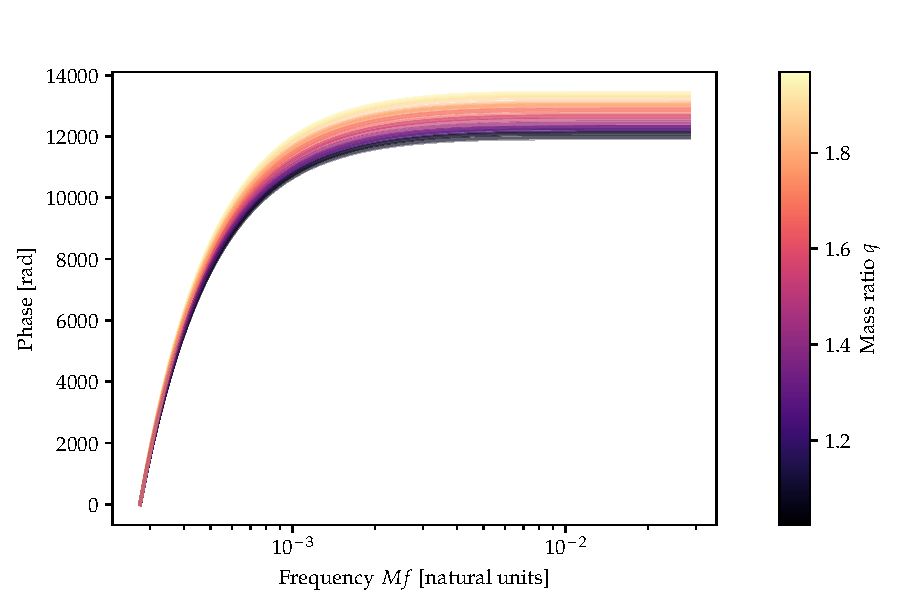
\includegraphics[width=.95\textwidth]{figures/native_phases}
    \label{fig:native_phases}
    \end{figure}
\end{frame}

\end{document}
